\documentclass[a4paper, 12pt]{article}
\usepackage[utf8]{inputenc}
\usepackage[T1, T2A]{fontenc}
\usepackage[a4paper, top=2cm, bottom=2cm, left=1cm, right=1cm, marginparwidth=1.75cm]{geometry}
\usepackage{graphicx}
\usepackage{amsmath}
\usepackage{amssymb}
\usepackage{amsfonts}
\usepackage{indentfirst}
\usepackage[english, russian]{babel}
\usepackage[section,above,below]{placeins}
\usepackage{pdfpages} 
\usepackage{svg}
\usepackage[colorlinks,urlcolor=blue]{hyperref}
\usepackage{multirow}

\begin{document}

\begin{table}[h]\begin{center}  \begin{tabular}[t]{|c|l|c|c|c|c|c|}\hline
    \multicolumn{2}{|c|}{Область и метод} & 5 & 6 & 7 & 8&9 \\ \hline
    \multirow{3}{*}{1}      
    & Метод 1     &   &   &   &  & \\ \cline{2-7} 
                            & Метод 1     &   &   &   &  & \\ \cline{2-7} 
                            & Метод 2     &   &   &   &   &\\ \hline
    \multirow{3}{*}{2}     
     & Метод 1     &   &   &   &  & \\ \cline{2-7} 
                            & Метод 1     &   &   &   &  & \\ \cline{2-7} 
                            & Метод 2     &   &   &   &  & \\ \hline
    \multirow{3}{*}{3}      
    & Метод 1     &   &   &   &  & \\ \cline{2-7} 
                            & Метод 1     &   &   &   &  & \\ \cline{2-7} 
                            & Метод 2     &   &   &   &  & \\ \hline
    \end{tabular}\end{center}\end{table}    
    
    \begin{table}[h]\begin{center}  \begin{tabular}[t]{|c|l|c|c|c|c|c|}\hline
        \multicolumn{2}{|c|}{Область и метод} & 5 & 10 & 20 & 30 & 40 \\ \hline
        \multirow3*1
        & Метод 1 (L = 0,81) & 0,3522478  & 0,3521968  & 0,3521968  & 0,3521968 & 0,3521968  \\ \cline{2 - 7} 
        & Метод 1 (L = 3,14) & 11,6239313  & 11,6239295  & 11,6239295  & 11,6239295 & 11,6239295  \\ \cline{2 - 7} 
        & Метод 2     & 0,0246687  & 0,0069362  & 0,0051544  & 0,0035962 & 0,0027198\\ \hline
        \multirow3*2
        & Метод 1 (L = 1,75) & 0,6125370  & 0,6125370  & 0,6125233  & 0,6125233 & 0,6074520  \\ \cline{2 - 7} 
        & Метод 1 (L = 3,34) & 2,2315009  & 2,2315009  & 2,2315009  & 2,2314973 & 2,2314973  \\ \cline{2 - 7} 
        & Метод 2     & 0,0117991  & 0,0036295  & 0,0028341  & 0,0026952 & 0,0025366\\ \hline
        \multirow3*3
        & Метод 1 (L = 2,82) & 3,8047554  & 3,8047554  & 3,8047554  & 3,8047554 & 3,8111539  \\ \cline{2 - 7} 
        & Метод 1 (L = 0,87) & 0,5273033  & 0,5273033  & 0,5273033  & 0,5273033 & 0,5273033  \\ \cline{2 - 7} 
        & Метод 2     & 0,0102984  & 0,0085362  & 0,0101249  & 0,0109433 & 0,0106923\\ \hline
        \end{tabular}\end{center}\end{table}
    



        \begin{figure}[!h]
            \begin{minipage}[h]{0.49\linewidth}
              \center{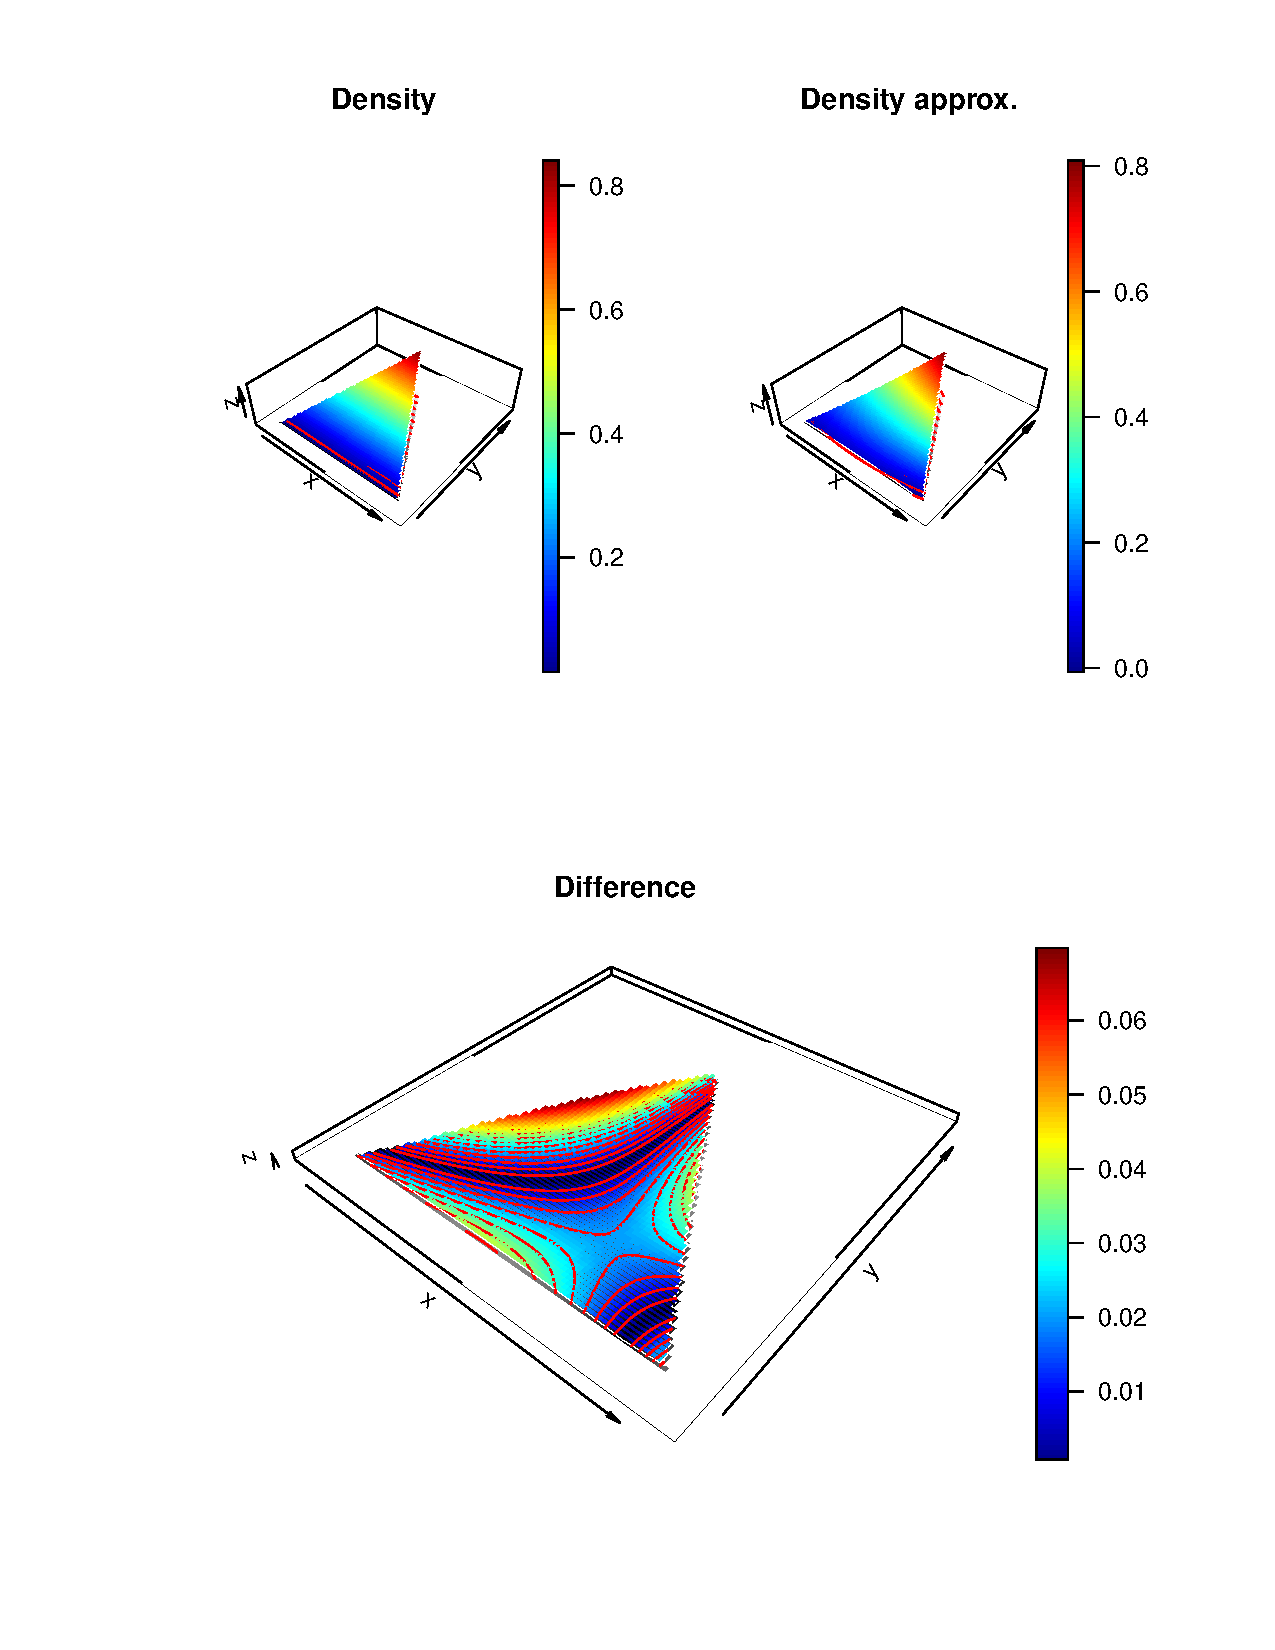
\includegraphics[width=0.95\linewidth]{f22.pdf}}
            \end{minipage}
            \hfill
            \begin{minipage}[h]{0.49\linewidth}
              \center{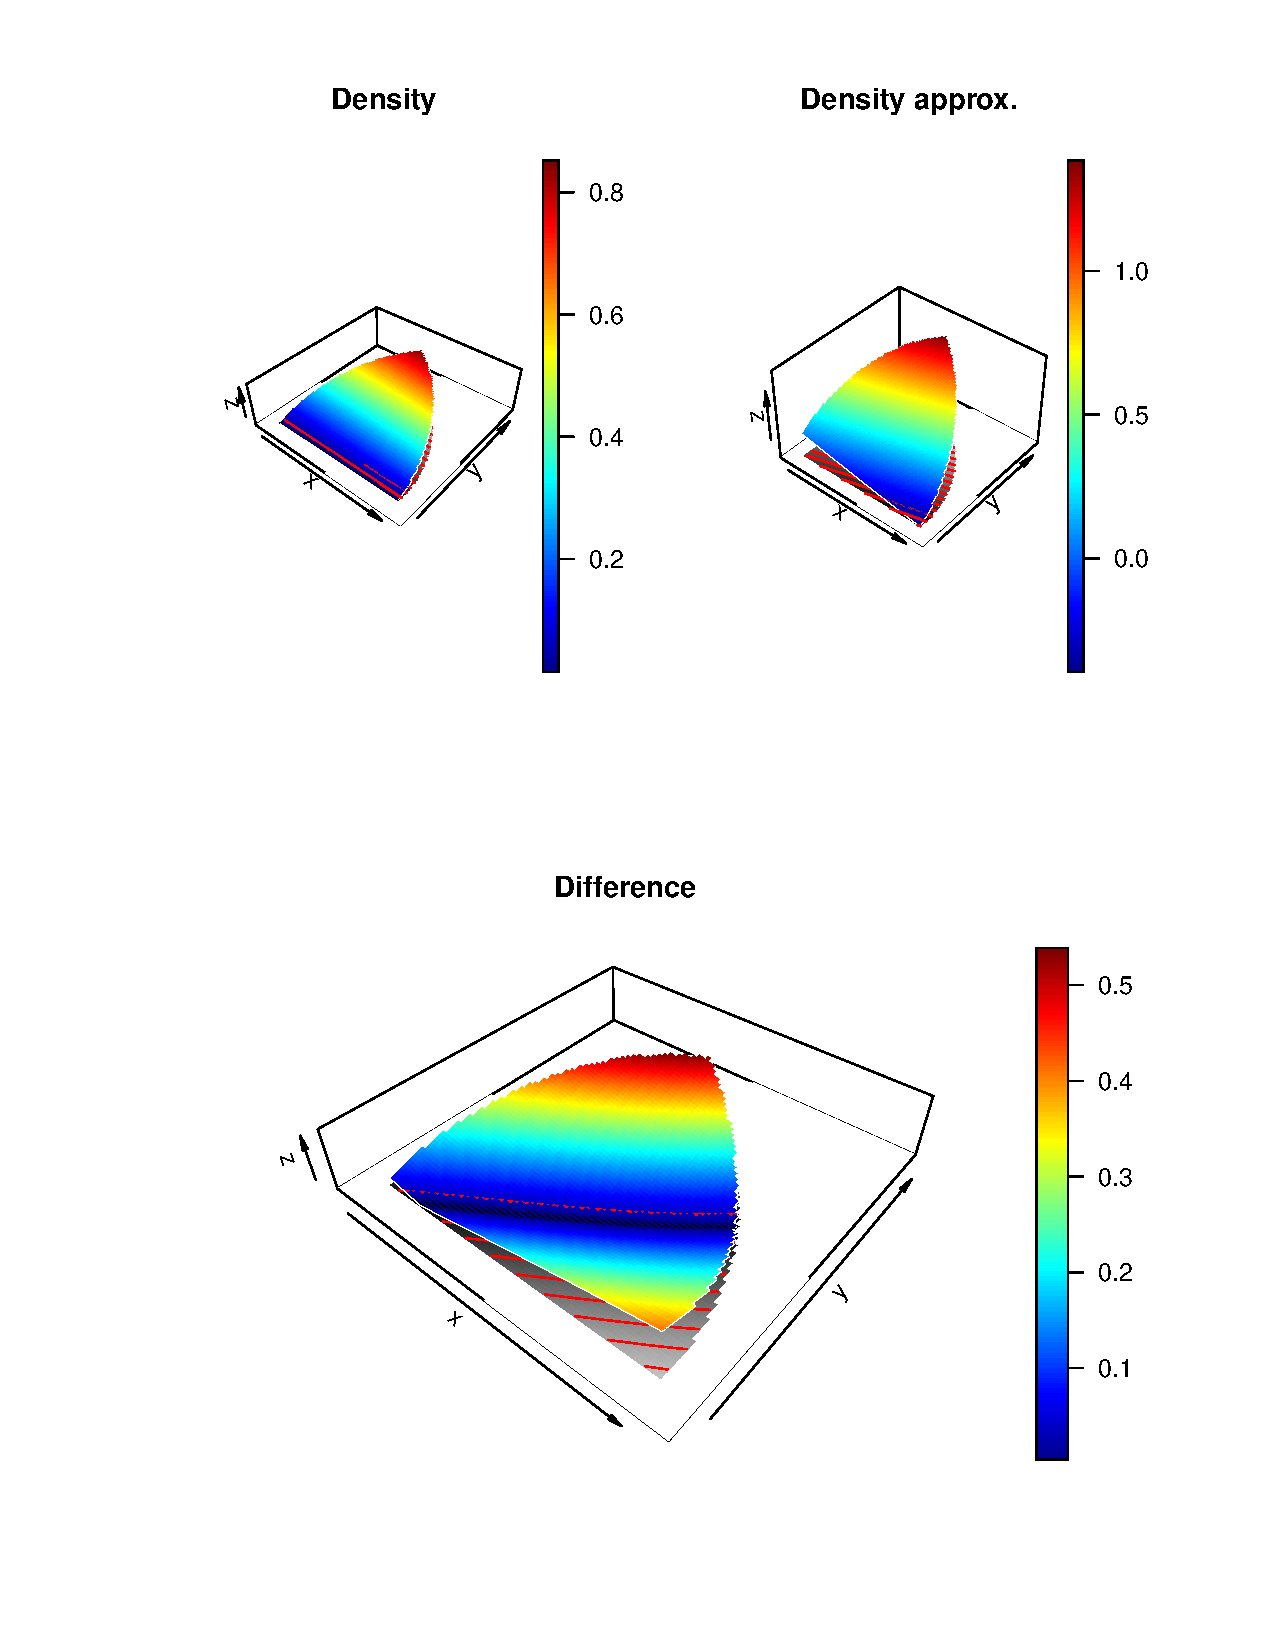
\includegraphics[width=0.95\linewidth]{f24.pdf}}
            \end{minipage}
            \caption{Для $f_2$}
            \label{ris:image1}
          \end{figure}



\end{document}